\textbf{7.1.} 一均匀磁化棒直径为 $10\mathrm{mm}$ , 长为 $30\mathrm{mm}$ , 磁化强度为 $1200\mathrm{A / m}$ . 试求它的磁矩.

\vfill

\textbf{7.2.} 一细长的均匀磁化棒, 磁化强度为 M, M 沿棒长方向, 如图 7.2(1) 所示. 试分别求图中 1 至 7 各点的磁场强度 H 和磁感强度 B.

图7.2(1)

图7.2(2)
\begin{center}
    
\includegraphics[width=0.5\linewidth]{figures/fig_7_2_1.jpg}
\end{center}
\begin{center}
    
\includegraphics[width=0.5\linewidth]{figures/fig_7_2_2.jpg}
\end{center}

\vfill

\newpage

\textbf{7.3.} 一铁环均匀磁化, 磁化强度为 M, M 沿环的方向; 环上有一很窄的空气隙, 如图 7.3 所示. 已知环的横截面的半径比环长小很多, 试分别求图中 1、2 和 3 等点的磁场强度 H 和磁感强度 B.

\vfill

\textbf{7.4.} 一磁棒均匀磁化, 磁化强度沿棒长方向. 试证明: 在棒的中垂面上, 棒表面附近内外的 1 和 2 两点(图 7.4) 的磁场强度相等. 这两点的磁感强度相等吗?
\begin{center}
    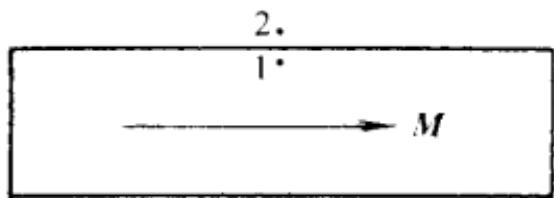
\includegraphics[width=0.5\linewidth]{figures/fig_7_4.jpg}
\end{center}

\vfill

\newpage

\textbf{7.5.} 一半径为 $R$ 、厚为 $\delta$ 的圆形薄磁片(磁壳)均匀磁化, 磁化强度为 $M, M$ 与两面垂直, 如图 7.5 所示, 图中 1、2、3 等点分别在磁片中心和磁片两面外靠近中心处. 试分别用(1)分子电流观点和(2)磁荷观点求这三点的磁感强度 $B$ 和磁场强度 $H$ .

(1) 立体图

(2) 侧视图
\begin{center}
    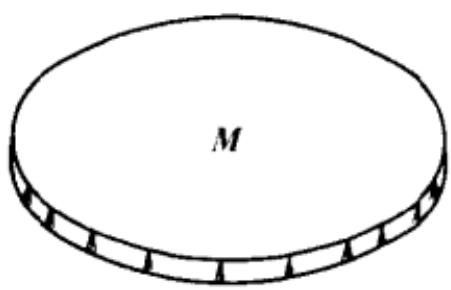
\includegraphics[width=0.5\linewidth]{figures/fig_7_5_1.jpg}
\end{center}
\begin{center}
    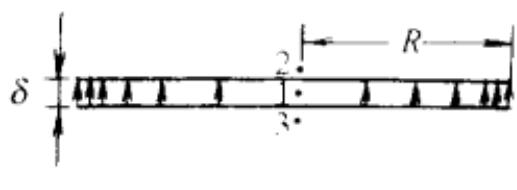
\includegraphics[width=0.5\linewidth]{figures/fig_7_5_2.jpg}
\end{center}

\vfill

\textbf{7.6.} 用5号吕臬古做的圆柱形磁铁，直径为 $10\mathrm{mm}$ ，长为 $100\mathrm{mm}$ ，均匀磁化后磁极化强度为 $1.2\mathrm{Wb / m^2}$ 。试求：(1)它两端的磁极强度 $q_{\mathrm{m}}$ ；(2)它的磁矩 $m$ 和磁偶极矩 $p_{\mathrm{m}}$ ；(3)当它放在磁感强度为 $\pmb{B}$ 的外磁场中， $\pmb{B}$ 与它垂直， $B = 10\mathrm{Gs}$ 时，它所受的力矩；(4)已知该磁铁的矫顽力为 $H_{\mathrm{C}} = 4.4\times 10^{4}\mathrm{A / m}$ ，上述外磁场的 $\pmb{H}$ 的大小与 $H_{\mathrm{C}}$ 之比。

\vfill

\newpage

\textbf{7.7.} 一磁铁棒长 $5.0\mathrm{cm}$ , 横截面积为 $1.0\mathrm{cm}^2$ , 密度为 $7.9\mathrm{g/cm}^3$ . 设棒内所有铁原子的磁矩都沿棒长方向整齐排列, 每个铁原子的磁矩为 $1.8 \times 10^{-23}\mathrm{A} \cdot \mathrm{m}^2$ . 已知铁的原子量为 55.85, 阿伏伽德罗常量为 $6.022 \times 10^{23}(\mathrm{mol})^{-1}$ . (1) 试求这铁磁棒的磁矩和磁偶极矩; (2) 当这铁磁棒处在 $B = 1.5\mathrm{T}$ 的外磁场中并与 $\pmb{B}$ 垂直时, $\pmb{B}$ 使它转动的力矩有多大?

\vfill

\textbf{7.8.} 一均匀磁化的圆柱形磁棒, 直径为 25mm, 长为 75mm, 磁矩为 $12A \cdot m^{2}$ . 试求它表面上磁化面电流密度的大小.

\vfill

\newpage

\textbf{7.9.} 真空中有一磁棒长为 $l$ ，磁极强度为 $q_{\mathrm{m}}$ ，试证明：它在很远处产生的磁感强度 $\pmb{B}$ 的分量为

$$
B _ {r} = \frac {q _ {\mathrm{m}} l \cos \theta}{2 \pi r ^ {3}}, \quad B _ {\theta} = \frac {q _ {\mathrm{m}} l \sin \theta}{4 \pi r ^ {3}}
$$

式中 $r(\gg l)$ 是棒中心到场点 $P$ 的距离， $\theta$ 是 $r$ 与棒长之间的夹角[图7.9(1)]， $B_r$ 和 $B_\theta$ 分别是 $\pmb{B}$ 在 $\pmb{r}$ 方向上和 $\theta$ 方向上的分量.

图7.9(1)

图7.9(2)
\begin{center}
    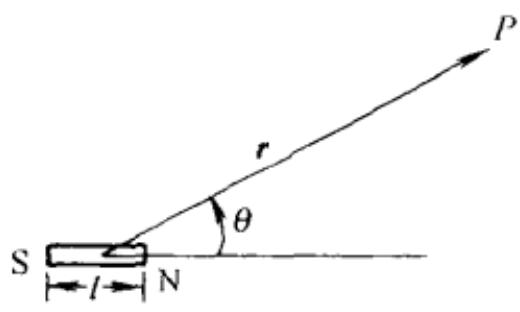
\includegraphics[width=0.5\linewidth]{figures/fig_7_9_1.jpg}
\end{center}
\begin{center}
    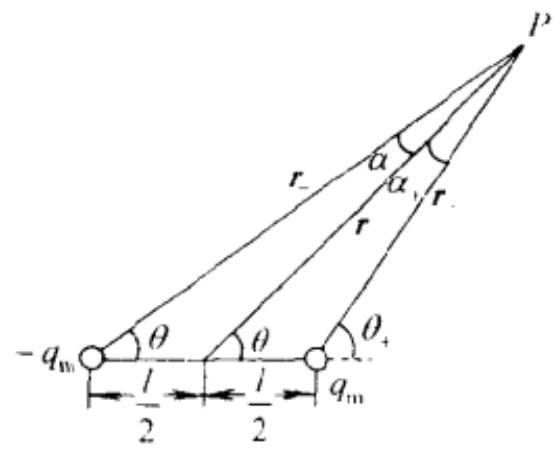
\includegraphics[width=0.5\linewidth]{figures/fig_7_9_2.jpg}
\end{center}

\vfill

\textbf{7.10.} 一平面线圈的面积为 S, 载有电流 I, 试证明: 它在很远处产生的磁感强度 B 的分量为


$$
B _ {r} = \frac {\mu_ {0} I S \cos \theta}{2 \pi r ^ {3}}, \quad B _ {\theta} = \frac {\mu_ {0} I S \sin \theta}{4 \pi r ^ {3}}
$$

式中 $r(r \gg \sqrt{S})$ 是线圈中心到场点 $P$ 的距离, $\theta$ 是 $r$ 与线圈平面的法线之间的夹角(图7.10), $B_r$ 和 $B_\theta$ 分别是 $\pmb{B}$ 在 $\pmb{r}$ 方向上和 $\theta$ 方向上的分量.[提示:与前面7.9题对比]
\begin{center}
    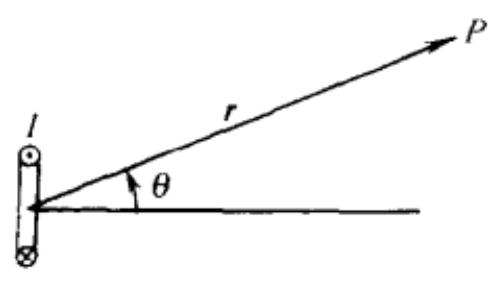
\includegraphics[width=0.5\linewidth]{figures/fig_7_10.jpg}
\end{center}

\vfill

\newpage

\textbf{7.11.} 一圆磁片(磁壳)的半径为 R，厚为 l，片的两面均匀分布着磁荷，磁荷量的面密度分别为 $\sigma_{m}$ 和 $-\sigma_{m}$ ，如图 7.11 所示。试求轴线上离圆片中心为 r 处 P 点的磁势 $U_{m}$ 和磁场强度 H。

(1) 立体图

(2) 侧面图
\begin{center}
    
\includegraphics[width=0.5\linewidth]{figures/fig_7_11_1.jpg}
\end{center}
\begin{center}
    
\includegraphics[width=0.5\linewidth]{figures/fig_7_11_2.jpg}
\end{center}

\vfill

\textbf{7.12.} 一永磁薄圆片, 半径为 $R = 1.0 \mathrm{~cm}$ , 其磁化方向与它的轴线平行. 测得轴线上离片中心为 $r = 10 \mathrm{~cm}$ 处的磁感强度为 $B = 30 \mu \mathrm{T}$ . 试计算这圆磁片边缘的磁化电流 $I_{\mathrm{m}}$ .

\vfill

\newpage

\textbf{7.13.} (1) 半径为 $R$ 的圆线圈载有电流 $I$ , 试求它在磁感强度为 $\pmb{B}$ 的均匀外磁场中所受的力矩 $\pmb{M}$ ; (2) 半径为 $R$ 的圆磁片(磁壳), 厚为 $l$ , 两面均匀分布着磁荷, 磁荷量的面密度分别为 $\sigma_{\mathrm{m}}$ 和 $-\sigma_{\mathrm{m}}$ , 试求它在磁感强度为 $\pmb{B}$ 的均匀外磁场中所受的力矩 $\pmb{M}'$ ; (3) 若 $\pmb{M}' = \pmb{M}$ , 则圆磁片就叫做圆电流的等效磁壳. 试求圆电流与它的等效磁壳的关系.

\vfill

\textbf{7.14.} 用磁荷观点处理一些问题,有时有方便之处.根据这种观点,磁荷之间的相互作用力遵守库仑定律,即磁荷量 $dq_{m}$ 在距离 r 处产生的磁场强度和磁势分别为

$$
\mathrm{d} \boldsymbol {H} = \frac {1}{4 \pi \mu_ {0}} \frac {\mathrm{d} q _ {\mathrm{m}}}{r ^ {3}} \boldsymbol {r}, \quad \mathrm{d} U _ {\mathrm{m}} = \frac {1}{4 \pi \mu_ {0}} \frac {\mathrm{d} q _ {\mathrm{m}}}{r}
$$

圆电流

同磁片

一个半径为 $R$ 的圆电流 $I$ , 可以看成是半径相同的一个薄磁片, 片的两面分别均匀地分布着面密度为 $\sigma_{\mathrm{m}}(\mathrm{N}$ 极) 和 $-\sigma_{\mathrm{m}}(\mathrm{S}$ 极) 的磁荷量, 如图 7.14 所示. 当片的厚度 $\delta \to 0$ , 面密度 $\sigma_{\mathrm{m}} \to \infty$ , 而 $\sigma_{\mathrm{m}} \delta =$ 常量时, 这种磁片就叫做该电流的等效磁壳. (1) 试求薄圆磁片轴线上离中心为 $r$ 处的磁场强度 $H$ ; (2) 把所得结果与圆电流在轴线上产生的 $H$ 比较, 两者关系如何? (3) 以圆心为极点、轴线为极轴取极坐标系, 空间任一点 $P$ 的坐标为 $r$ , $\theta$ ( $\theta$ 是圆心到 $P$ 的联线与极轴的夹角), 试求薄圆磁片在 $r \gg R$ 处 $P$ 点产生的磁势 $U_{\mathrm{m}}$ , 然后由磁场强度 $H$ 与 $U_{\mathrm{m}}$ 的关系 $H = -\nabla U_{\mathrm{m}}$ 求 $H$ . 这样求得的 $H$ 也就是相应圆电流产生的磁场强度.
\begin{center}
    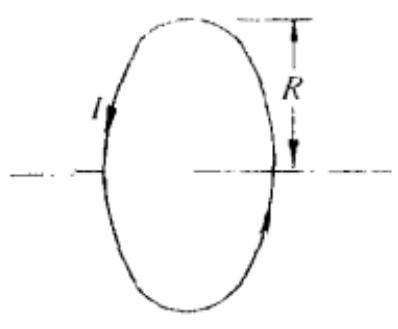
\includegraphics[width=0.5\linewidth]{figures/fig_7_14_1.jpg}
\end{center}
\begin{center}
    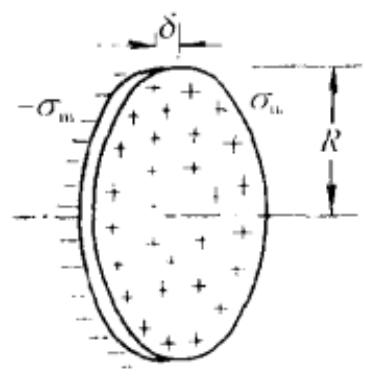
\includegraphics[width=0.5\linewidth]{figures/fig_7_14_2.jpg}
\end{center}

\vfill

\newpage

\textbf{7.15.} (1)一个圆柱形磁棒长为 $l$ ，横截面的半径为 $R$ ，它可以看作是两端面上均匀分布着磁荷的圆柱体，N、S两端面上面磁荷密度分别为 $\sigma_{\mathrm{m}}$ 和 $-\sigma_{\mathrm{m}}$ ，如图7.15(1)所示。试分别求轴线上离中心为 $x_{1}$ （棒内）和 $x_{2}$ （棒外）处的磁场强度 $H$ ；(2)一密绕螺线管长为 $l$ ，横截面的半径为 $R$ ，共有 $N$ 匝，每匝电流为 $I$ 。试分别求管内外轴线上的磁场强度 H;(3) 将以上两者的 H 作一比较.

\vfill

\textbf{7.16.} 一螺线管由表面绝缘的细导线在纸筒上密绕而成,导线中通有电流;另有一均匀磁化的磁棒.试定性地画出它们的 H 线和 B 线.

\vfill

\newpage

\textbf{7.17.} 一半径为 $R$ 的无限长螺线管，由表面绝缘的细导线密绕而成，单位长度的匝数为 $n$ ，管内充满磁导率为 $\mu$ 的均匀磁介质。当导线中载有电流 $I$ 时，设 $I$ 的右旋进方向上的单位矢量为 $e_I$ 。试求：(1)管内介质中的磁场强度 $H$ 、磁感强度 $B$ 和磁化强度 $M$ ；(2)介质表面的磁化面电流密度 $k_{\mathrm{m}}$ ， $I$ 和 $k_{\mathrm{m}}$ 产生的磁感强度。

\vfill

\textbf{7.18.} 一无限长圆柱形直铜线, 横截面的半径为 $R$ , 线外包有一层相对磁导率为 $\mu_r$ 的均匀磁介质, 层厚为 $d$ , 导线中通有电流 $I, I$ 均匀分布在横截面上. 试求: (1) 离轴线为 $r$ 处的磁场强度 $\pmb{H}$ 和磁感强度 $\pmb{B}$ 的大小; (2) 磁介质内、外表面上的磁化电流.

\vfill

\newpage

\textbf{7.19.} 在空气 $(\mu_{\mathrm{r}} = 1)$ 和软铁 $(\mu_{\mathrm{r}} = 7000)$ 的交界面上，软铁上的磁感强度与交界面法线的夹角为 $85^{\circ}$ ，试求空气中磁感强度与交界面法线的夹角。

\vfill

\textbf{7.20.} 磁导率分别为 $\mu_{1}$ 和 $\mu_{2}$ 的两种均匀磁介质各充满一半空间，它们的交界面是一无限大平面，一条外皮绝缘的无穷长直导线载有电流 $I$ ，正处在交界面上.试求 $I$ 所产生的磁感强度.

\vfill

\newpage

\textbf{7.21.} 一半径为 R 的磁介质球均匀磁化, 磁化强度为 M, 如图 7.21 所示. (1) 根据分子电流的观点, 试求它的磁化电流和磁矩; (2) 根据磁荷观点, 试求它的磁荷和磁偶极矩.

\vfill

\textbf{7.22.} 一介质球均匀磁化, 磁化强度为 M. 试求沿 M 的直径上离球心为 r 处的磁感强度.

\vfill

\newpage

\textbf{7.23.} 中子星是超新星爆发所产生的一种天体, 具有很强的磁场. 假设中子星是由中子密集构成的球体, 它的磁场来自中子的磁矩 $\mu_{n}, \mu_{n}$ 都沿同一方向排列. 已知中子的半径为 $a = 8 \times 10^{-16} ~m$ , 中子磁矩的大小为 $\mu_{n} = 9.66 \times 10^{-27} ~A \cdot m^{2}$ . 试求中子星表面磁场最强处磁感强度的值.

\vfill

\textbf{7.24.} 一块很大的铁磁介质, 相对磁导率为 $\mu_{\mathrm{r}} = 200$ , 内部有磁感强度为 $B = 2.0\mathrm{T}$ 的磁场. 在它里面有两个小空穴, 一个是两面垂直于 $B$ 的薄圆盘形, 另一个是平行于 $B$ 的细长针形. 试分别求这两空穴中心的磁场强度 $H$ .

\vfill

\newpage

\textbf{7.25.} 有些铁氧体(如锰镁铁氧体和锂锰铁氧体)的磁滞回线接近矩形,称为矩磁材料,它们在电流的磁场中磁化后,当电流变到零时,便处在 H=0 处的 $B_{r}$ 或 $-B_{r}$ 这两个剩磁状态之一,如图 7.25(1) 所示.这个特点符合电子计算机的二进位制,可以让其中一个状态代表 0,另一个状态代表 1,因此,在电子计算机里用作存储元件.一矩形材料做的磁芯存储器为环形,其外直径为 0.8mm,它的矫顽力为 $H_{c}=2Oe$ ;在它的轴线上有一条长直导线,通过导线中的电流 I 以改变它所处的状态.设它处在剩磁状态之一 $(B_{r})$ ,其方向如图 7.25(2) 所示.现在要用导线中的脉冲电流 I 使环内磁场全部翻转到另一剩磁状态 $(-B_{r})$ ,试问 I 的峰值至少要多大?

图7.25(1)

图7.25(2)
\begin{center}
    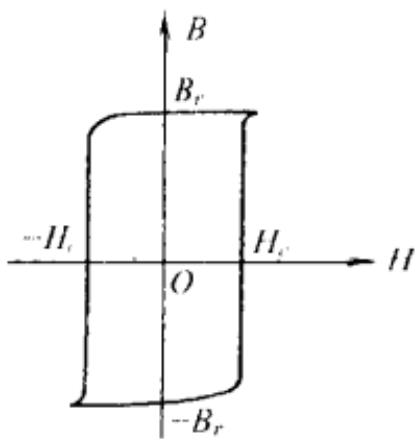
\includegraphics[width=0.5\linewidth]{figures/fig_7_25_1.jpg}
\end{center}
\begin{center}
    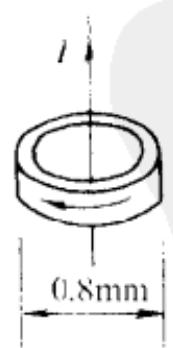
\includegraphics[width=0.5\linewidth]{figures/fig_7_25_2.jpg}
\end{center}

\vfill

\textbf{7.26.} 据测量得出,地球的磁矩为 $m = 8.0 \times 10^{22} \, A \cdot m^{2}$ . (1) 如果在地磁赤道上套一个铜环,在这环里通以电流 I,使它的磁矩等于地球的磁矩,已知地球的半径为 6400 km. 试求 I 的值; (2) 如果这电流的磁矩与地球的磁矩正好方向相反,试问这样能不能完全抵消地球表面的磁场?

\vfill

\newpage

\textbf{7.27.} 地磁场可以近似地看做是位于地心的一个磁偶极子产生的，在地磁纬度 $45^{\circ}$ 处，地磁的水平分量平均为0.23Oe.已知地球的平均半径为 $6370\mathrm{km}$ ，试求上述磁偶极子的磁矩.

\vfill

\textbf{7.28.} 地球的磁场可以近似地看做是位于地心的一个磁偶极子产生的, 如图 7.28 所示. 试证明: (1) 磁倾角(地磁场的方向与当地水平面之间的夹角) i 与地磁纬度 $\varphi$ 的关系为 $\tan i = 2\tan\varphi$ ; (2) 地磁北极处的地磁竖直分量等于地磁赤道上地磁水平分量的两倍.

\vfill

\newpage

\textbf{7.29.} 根据经典模型, 氢原子处在基态时, 电子环绕氢核(质子)作匀速圆周运动, 轨道半径为 $5.29 \times 10^{-11} \mathrm{~m}$ , 频率为 $6.58 \times 10^{15} \mathrm{~Hz}$ . 已知电子电荷量的大小为 $1.60 \times 10^{-19} \mathrm{C}$ . 试求电子沿轨道运动的磁矩 $\mu_{\mathrm{B}}$ (这种轨道运动磁矩通常叫做玻尔

磁子)和磁偶极矩 $p_{B}$ .

\vfill

\textbf{7.30.} 已知质子的电荷量为 $1.60 \times 10^{-19} \mathrm{C}$ , 磁矩为 $1.41 \times 10^{-26} \mathrm{~A} \cdot \mathrm{m}^{2}$ , 质子的体积非常小。(1) 在质子磁矩的中垂面上离质子为 $0.529 \mathring{\mathrm{A}} (1 \mathring{\mathrm{A}} = 10^{-10} \mathrm{~m})$ 处, 质子所产生的电场强度和磁感强度各有多大? (2) 按照经典模型, 氢原子处在基态时, 电子在上述距离处环绕氢核(质子)作匀速圆周运动, 速率为 $2.19 \times 10^{6} \mathrm{~m/s}$ . 试求电子受到的洛伦兹力与库仑力之比.

\vfill

\newpage

\textbf{7.31.} 一螺绕环由表面绝缘的导线在铁环上密绕而成,每厘米绕有10匝;当导线中载有2.0A的电流时,测得铁环内部的磁感强度为1.0T.试求:(1)铁环内部的磁场强度H;(2)铁环的磁化强度M和相对磁导率 $\mu_{r}$ .

\vfill

\textbf{7.32.} 一铁环中心线的周长为 $30\mathrm{cm}$ , 横截面积为 $1.0\mathrm{cm}^2$ , 在环上紧密地绕有 300 匝表面绝缘的导线; 当导线中通有 $32\mathrm{mA}$ 的电流时, 测得通过环的横截面的磁通量为 $2.0 \times 10^{-6}\mathrm{Wb}$ . 试求: (1) 铁环内部磁感强度的大小 $B$ 和磁场强度的大小 $H$ ; (2) 铁环的磁化强度的大小 $M$ ; (3) 铁环的磁化率 $\chi_{\mathrm{m}}$ 、相对磁导率 $\mu_{\mathrm{r}}$ 和磁导率 $\mu$ .

\vfill

\newpage

\textbf{7.33.} 一铁心螺绕环由表面绝缘的导线在铁环上密绕而成, 环的中心长度为 $600\mathrm{mm}$ , 横截面积为 $1000\mathrm{mm}^2$ . 现在要在环内部产生 $B = 1.0\mathrm{T}$ 的磁感强度, 由铁的 $B - H$ 曲线得这时铁的 $\mu_{\mathrm{r}} = 795$ , 试求所需的安匝数. 如果在铁环上有一个 $2.0\mathrm{mm}$ 宽的空气隙, 试求所需的安匝数.

\vfill

\textbf{7.34.} 一铁环中心线的半径为 $200\mathrm{mm}$ , 横截面积为 $150\mathrm{mm}^2$ , 在它上面绕有表面绝缘的导线 $N$ 匝, 导线中通有电流 $I$ . 在铁环上有一个空气隙, 宽为 $1.0\mathrm{mm}$ . 现在要在空气隙内产生 $B = 0.50\mathrm{T}$ 的磁感强度, 由铁的 $B - H$ 曲线得出这时铁的 $\mu_{\mathrm{r}} = 250$ , 试求所需的安匝数 $NI$ .

\vfill

\newpage

\textbf{7.35.} 一铁环中心线的半径为 $R = 20\mathrm{cm}$ , 横截面是边长为 $4.0\mathrm{cm}$ 的正方形.

环上绕有 500 匝表面绝缘的导线, 导线中载有 1.0A 的电流, 这时铁的相对磁导率为 $\mu_{r}=400$ . (1) 试求通过铁环的横截面的磁通量 $\Phi$ ; (2) 如果在这铁环上锯开一个宽为 1.0mm 的空气隙, 试问通过铁环的横截面的磁通量减少了多少?

\vfill

\textbf{7.36.} 一铁环中心线的直径为 $D = 40\mathrm{cm}$ ，环上均匀地绕有一层表面绝缘的导线，导线中通有不变的电流。若在这铁环上锯一个宽为 $1.0\mathrm{mm}$ 的空气隙，则通过环的横截面的磁通量为 $3.0 \times 10^{-4}\mathrm{Wb}$ ；若空气隙的宽度为 $2.0\mathrm{mm}$ ，则通过环的横截面的磁通量为 $2.5 \times 10^{-4}\mathrm{Wb}$ 。略去漏磁，试求这铁环的磁导率。

\vfill

\newpage

\textbf{7.37.} 一个利用空气间隙获得较强磁场的装置如图7.37所示，铁心是相对磁导率为 $\mu_{2} = 5000$ 的硅钢，它的中心线的长度为 $l_{1} = 500\mathrm{mm}$ ，空气隙的宽度为 $l_{2} = 20\mathrm{mm}$ 。要在空气隙中得到 $B = 3000\mathrm{Gs}$ 的磁场，试求绕在铁心上的线圈的安匝数 $NI$ 。

\vfill

\textbf{7.38.} 某电钟里有一铁心线圈, 已知铁心的磁路长为 $14.4 \mathrm{~cm}$ , 空气隙宽为 $2.0 \mathrm{~mm}$ , 铁心的横截面积为 $0.60 \mathrm{~cm}^{2}$ , 铁心的相对磁导率为 $\mu_{\mathrm{r}} = 1600$ . (1) 现在要使通过空气隙的磁通量为 $4.8 \times 10^{-6} \mathrm{~Wb}$ , 试求绕在铁心上的线圈的安匝数 $N I$ ; (2) 若线圈两端电压为 $220 \mathrm{~V}$ , 线圈消耗的功率为 $2.0 \mathrm{~W}$ , 试求线圈的匝数.

\vfill

\newpage

\textbf{7.39.} 一永磁铁环的平均直径为 $20\mathrm{cm}$ ，环上有一宽为 $2.0\mathrm{mm}$ 的空气间隙，间隙内的磁感强度为 $40\mathrm{mT}$ . 略去间隙边缘的漏磁，试估算间隙内和磁铁内磁场强度

的值.

\vfill

\textbf{7.40.} 一磁偶极子的磁偶极矩为 $p_{\mathrm{m}}$ ，处在磁场强度为 $\pmb{H}$ 的非均匀外磁场中， $p_{\mathrm{m}}$ 与 $\pmb{H}$ 平行或逆平行。（1）试证明，它受磁场 $\pmb{H}$ 的作用力 $f$ 的大小为 $f = p_{\mathrm{m}}\left|\frac{\partial H}{\partial l}\right|$ ，式中 $\frac{\partial H}{\partial l}$ 是 $\pmb{H}$ 的大小沿 $p_{\mathrm{m}}$ 方向的微商；(2) $f$ 的方向如何？

\vfill

\newpage

\textbf{7.41.} 一永磁体的磁偶极子, 其磁矩为 m, 处在磁感强度为 B 的外磁场(静磁场)中. 试证明, 它的磁势能为 $W_{m} = -m \cdot B$ .

\vfill

\textbf{7.42.} 原子和分子的磁矩一般是玻尔磁子 $\mu_{B}=\frac{e\hbar}{2m}=9.274\times10^{-24}A\cdot m^{2}$ 的数量级. 试问: (1) 一个玻尔磁子在磁感强度为 B=10T 的外磁场中, 当 $\mu_{B}$ 与 B 逆平行时, 它的势能是多少? (2) 这势能与室温下分子热运动的能量 (数量级为 kT) 比较, 哪个大? 大多少倍?

【解答】(1) $\mu_{B}$ 与B逆平行时,它的势能为

$$
\begin{array}{r l} W _ {\mathrm{m}} & = - \boldsymbol {\mu} _ {\mathrm{B}} \cdot \boldsymbol {B} = \mu_ {\mathrm{B}} B = 9. 2 7 4 \times 1 0 ^ {- 2 4} \times 1 0 = 9. 2 7 4 \times 1 0 ^ {- 2 3} (\mathrm{J}) \\ & = 5. 8 \times 1 0 ^ {- 4} (\mathrm{eV}) \end{array}
$$

(2)室温下分子热运动能量的数量级为

$$
\begin{array}{r l} E & = k T = 1. 3 8 \times 1 0 ^ {- 2 3} \times 3 0 0 = 4. 1 4 \times 1 0 ^ {- 2 1} (\mathrm{J}) \\ & = 2. 6 \times 1 0 ^ {- 2} (\mathrm{eV}) \end{array}
$$

可见 $E > W_{\mathrm{m}}$ ，比值为

$$
\frac {E}{W _ {\mathrm{m}}} = \frac {2 . 6 \times 1 0 ^ {- 2}}{5 . 8 \times 1 0 ^ {- 4}} = 4 5
$$
\begin{center}
    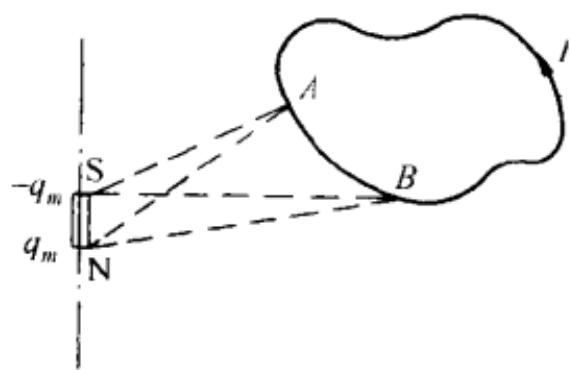
\includegraphics[width=0.5\linewidth]{figures/fig_7_42.jpg}
\end{center}

\vfill

\newpage

\textbf{7.43.} 载有电流 I 的导线是一条平面曲线，在同一平面内有一小磁棒，它两极的磁极强度（磁荷量）分别为 $q_{m}$ 和 $-q_{m}$ ，这导线上任何一段 AB（图 7.43）都将受到磁棒的作用力。试证明：这力对于转轴 NS 的力矩的大小为 $M = \frac{q_{m}I}{4\pi} (\cos \angle ANS + \cos \angle ASN - \cos \angle BNS - \cos \angle BSN)$ 。

\vfill

\textbf{7.44.} 在原点有一磁矩为 $m$ 的磁偶极子， $m = mk, m > 0, m$ 在 $r$ 处产生的磁感强度为

$$
\boldsymbol {B} = \frac {\mu_ {0}}{4 \pi r ^ {3}} \left[ \frac {3 (\boldsymbol {m} \cdot \boldsymbol {r}) \boldsymbol {r}}{r ^ {2}} - \boldsymbol {m} \right]
$$

另一圆电流 I, 半径为 a, 中心在 $(0,0,b)$ 处, 其轴线与 z 轴重合, 如图 7.44 所示. 试求它们之间的相互作用力.

\vfill

\newpage

\textbf{7.45.} 两磁偶极子在同一条直线 r. 试证明, 它们之间相互作用力的大小为 $f = 3p_{1}p_{2}/2\pi\mu_{0}r^{4}$ ; 在什么情况下它们互相吸引?

$$
p _ {1}
$$

$$
p _ {2}
$$
\begin{center}
    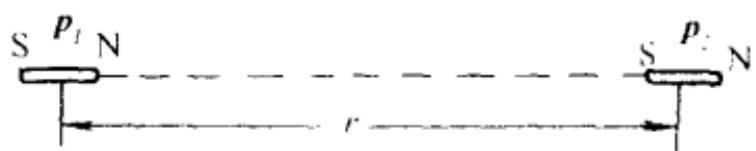
\includegraphics[width=0.5\linewidth]{figures/fig_7_45.jpg}
\end{center}

\vfill

\textbf{7.46.} 两磁偶极子的磁矩分别为 $m_{1}$ 和 $m_{2}, r$ 是从 $m_{1}$ 到 $m_{2}$ 的矢径. 试证明: $m_{1}$ 作用在 $m_{2}$ 上的力为

$$
f = \frac {3 \mu_ {0}}{4 \pi r ^ {5}} \left[ (m _ {1} \cdot r) m _ {2} + (m _ {2} \cdot r) m _ {1} + (m _ {1} + m _ {2}) r - \frac {5 (m _ {1} \cdot r) (m _ {2} \cdot r)}{r ^ {2}} r \right]
$$

\vfill

\newpage

\textbf{7.47.} 磁偶极矩分别为 $p_1$ 和 $p_2$ 的两个小磁针固定在一起，中心重合， $p_1$ 与 $p_2$ 的夹角为 $\theta = \theta_1 + \theta_2$ ，用细线拴住它们的重心，悬挂着使它们处在水平面内并可以自由转动。加上一个水平的均匀外磁场 $\pmb{B}$ ，当它们达到静止时， $p_1$ 和 $p_2$ 与 $\pmb{B}$ 的夹角分别为 $\theta_1$ 和 $\theta_2$ ，如图7.47(1)所示（图面是水平面）。试证明： $\frac{\sin\theta_1}{p_2} = \frac{\sin\theta_2}{p_1} = \frac{\sin\theta}{\sqrt{p_1^2 + p_2^2 + 2p_1p_2\cos\theta}}$

图7.47(1)
\begin{center}
    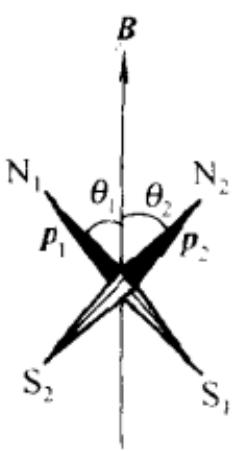
\includegraphics[width=0.5\linewidth]{figures/fig_7_47.jpg}
\end{center}

\vfill

\textbf{7.48.} 试论证: 在非铁磁质里的任一点, 磁感强度 B 的值(以高斯为单位)等于磁场强度 H 的值(以 Oe 为单位).

【论证】在国际单位制(SI)里,磁感强度 B 与磁场强度 H 的关系为

$$
B = \mu_ {\mathrm{r}} \mu_ {0} H\tag{1}
$$

其中 B 的单位为特斯拉(T), H 的单位为安/米(A/m), $\mu_{0}=4\pi\times10^{-7}H/m,\mu_{r}=1+\chi_{m}$ 是无量纲的纯数.

高斯(Gs)和奥斯特(Oe)分别是高斯单位制里磁感强度的单位和磁场强度的单位,它们与国际单位制的换算关系为

$$
\mathrm{IT} = 1 0 ^ {4} \mathrm{Gs}\tag{2}
$$

$$
1 \mathrm{A} / \mathrm{m} = \frac {4 \pi}{1 0 ^ {3}} \mathrm{Oe}\tag{3}
$$

当某点的磁感强度为 a 高斯时, 即

$$
B = a (\mathrm{Gs}) = a \times 1 0 ^ {- 4} (\mathrm{T})\tag{4}
$$

按式(1)，该点的磁场强度即为

$$
\begin{array}{r l} H = \frac {B}{\mu_ {\mathrm{r}} \mu_ {0}} & = \frac {a \times 1 0 ^ {- 4}}{4 \pi \times 1 0 ^ {- 7} \mu_ {\mathrm{r}}} = \frac {1 0 ^ {3}}{4 \pi} \frac {a}{\mu_ {\mathrm{r}}} (\mathrm{A/m}) \\ & = \frac {a}{\mu_ {\mathrm{r}}} \frac {1 0 ^ {3}}{4 \pi} \cdot \frac {4 \pi}{1 0 ^ {3}} (\mathrm{Oe}) = \frac {a}{\mu_ {\mathrm{r}}} (\mathrm{Oe}) \end{array}\tag{5}
$$

对于非铁磁介质来说， $\chi_{\mathrm{m}}$ 最大不过万分之三 $(3\times 10^{-4})$ 。因此，在万分之几的精确度范围内，有

$$
\mu_ {\mathrm{r}} = 1 + \chi_ {\mathrm{m}} \approx 1\tag{6}
$$

这时，式(5)便化为

$$
H = a (\mathrm{Oe})\tag{7}
$$

(4)、(7)两式表明:在该点,磁感强度 B 的值(以 Gs 为单位)等于磁场强度 H 的值(以 Oe 为单位).

【别解】在高斯单位制里，B与H的关系为

$$
B - \mu_ {\mathrm{r}} H\tag{8}
$$

因为在高斯单位制里，磁感强度 B 以 Gs 为单位，磁场强度 H 以 Oe 为单位，故由式(8)即可得出上述结论.

\vfill

\newpage
